\chapter{IACT Experiments}
\label{cta}

sensitivity in crab flux angeben

\section{The Current Generation}

Towards the end of the 1990s several third generation experiments were
proposed:
H.E.S.S and MAGIC, deriving from parts of the HEGRA collaboration, 
VERITAS from Whipple and the no longer operating CANGAROO from Adelaide and 
several japanese universities \cite{HILLAS201319}. All of these
were designed as stereoscopic imaging telescopes building on the progress made during the 
earlier experiments with two experiments located on each the north and the south hemisphere.

\subsection{Major Atmospheric Gamma Imaging Telescopes (MAGIC)}
MAGIC is a experiment nowadays operating as a stereo setup of two telescopes.
The two telescopes are located at La Palma and have a \SI{17}{\meter} diameter mirror setup each \cite{ALEKSIC201676}.

In the first phase MAGIC consisted of a single telescope, for differentiation usually
referred to as MAGIC-I. This first phase started 
operation in 2004 and had MAGIC-I be the largest IACT of its time.

The addition of MAGIC-2, the second mostly identical telescope, in 2009 marked the 
start of the second phase of the experiment and the transition to a third 
generation experiment \cite{2009arXiv0907.1211C}.
In the second phase MAGIC operates in the energy range from \SI{30}{\giga\eV}
up to \SI{100}{\TeV} \cite{magic_website}.

The DISP-method for the reconstruction of the event arrival direction 
was significantly improved by including timing information and showed better 
results for stereoscopy than the simple crossing of the main shower axis \cite{ALEKSIC2012435}.

A specialty of the MAGIC experiment lies in its ability to 
perform fast skews and thus react to gamma ray bursts after they have been observed 
by satellite experiments \cite{2003ICRC....5.2943B}.
This enabled the recent observation of the very first \si{\TeV}
gamma ray burst observed with IACTs \cite{collaboration2019teraelectronvolt}.


\subsection{Very Energetic Radiation Imaging Telescope Array System (VERITAS)}
VERITAS	was initially planned as a seven-telescope array, arranged in a diamond shape
\cite{WEEKES2002221}.

Eventually the collaboration settled 
with four telescopes. 
Each telescope covers a 3.5° FoV with a \SI{12}{\meter} diameter mirror and 
a 499 pixel PMT camera.

A relocation of telescope 1 in 2009 meant that the 
experiment made better use of the given area and its four telescopes,
improving the sensitivity by up to 30\% \cite{2009arXiv0912.3841P}.
The old and new layout can be seen in figure \ref{fig:veritas_relocation}.

The VERITAS collaboration mentions a lower threshold of \SI{100}{\giga\electronvolt}
with the four telescope setup.

\begin{figure}
	\center
	\captionsetup{width=0.9\linewidth}
	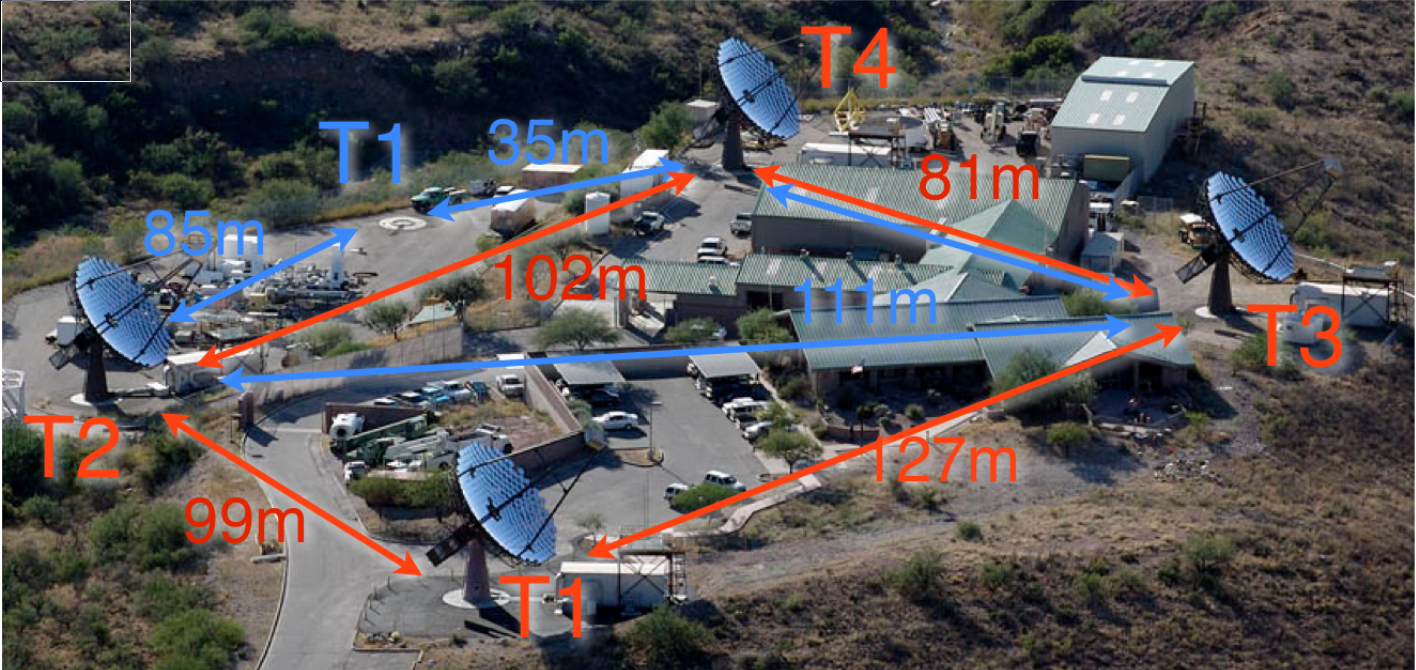
\includegraphics[width=.9\textwidth]{images/veritas_relocation.png}
	\caption{The VERITAS array layout after relocation of the first 
		telescope. The distances between the telescopes are 
		highlighted for the old(blue) and the new(red) array.
		In the old setup the telescopes T1, T2 and T4 were too closely
		located, making their measurements redundant.
	 	The image is taken from an official paper, that investigates
		the improved performance gained by relocating the telescope \cite{2009arXiv0912.3841P}.}
	\label{fig:veritas_relocation}
\end{figure}

Like MAGIC, VERITAS makes use of the DISP-method, especially at large zenith angles 
\cite{2015ICRC...34..771P}.

\subsection{High Energy Stereoscopic System (HESS)}

The HESS experiment consists of five telescopes and 
is - in contrast to MAGIC and VERITAS - operating in the southern 
Hemisphere, in Namibia.

A similar distinction in phase I and phase II as with MAGIC can be taken with 
HESS phase I consisting of four \SI{13}{\meter} diameter telescopes,
arranged at the edge of a square of \SI{120}{\meter} long sides \cite{HINTON2004331}.
These operated from 2004 to 2012 when the experiment went into phase II.

Phase II brought the larger, fifth telescope with the aim to lower the energy threshold
further. This $\SI{24}{\meter} \times \SI{32}{\meter}$-mirror telescope 
was placed in the middle of the other telescopes.
HESS operates at a similar energy range as MAGIC, stating a lower threshold as low as 
\SI{20}{\giga\electronvolt} \cite{vincent2005hess}.


\section{Next to come: The Cherenkov Telescope Array (CTA)}
\label{sec:cta}

The Cherenkov Telescope Array aims to be a next generation IACT experiment.
With two sites of operation, one for each hemisphere, and a number of different 
telescopes proposed, CTA is going to expand on the findings of the third 
generation experiments.

Like HESS in phase II, the CTA arrays are going to consist of different sized telescopes, namely
the Large Sized Telescope (LST, \SI{23}{\meter}), 
the Medium Sized Telescope (MST, \SI{12}{\meter}) 
and the Small Sized Telescope (SST, \SI{4.3}{\meter}).

Extensive Monte Carlo simulations have been performed to find optimal array arrangements
\cite{BERNLOHR2013171}.

The currently planned layouts at LaPalma and in Chile are shown in 
\ref{fig:cta_layout}.
The expected sensitivity compared against other currently operating
experiments is shown in figure \ref{fig:cta_performance}.

\begin{figure}[H]
	\center
	\captionsetup{width=0.9\linewidth}
	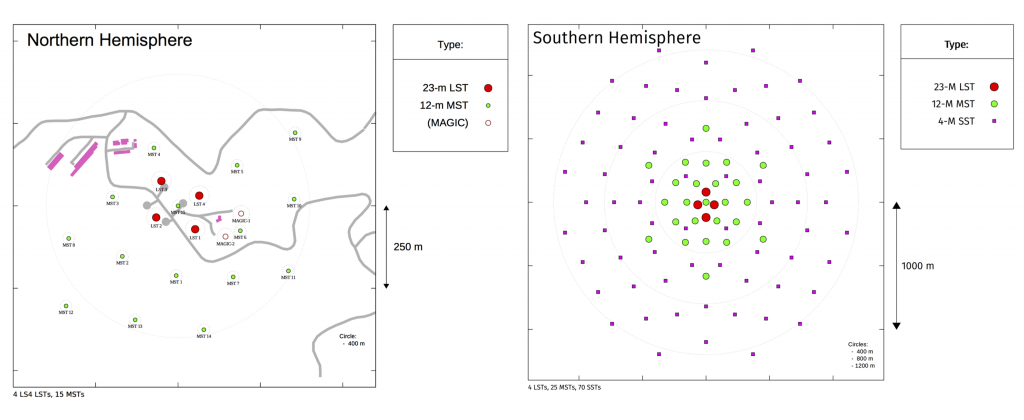
\includegraphics[width=0.9\textwidth]{images/cta_layout.png}
	\caption{
	Left: The array on the northern hemisphere. It will be build at LaPalma
	and feature only LSTs and MSTs.
	Right: The array at the southern hemisphere.
	It will consist of more telescopes and thus 
	work at a bigger energy range.
	The image is taken from the CTA-website \cite{cta_web}.}
	\label{fig:cta_layout}
\end{figure}

\begin{figure}[H]
	\center
	\captionsetup{width=0.9\linewidth}
	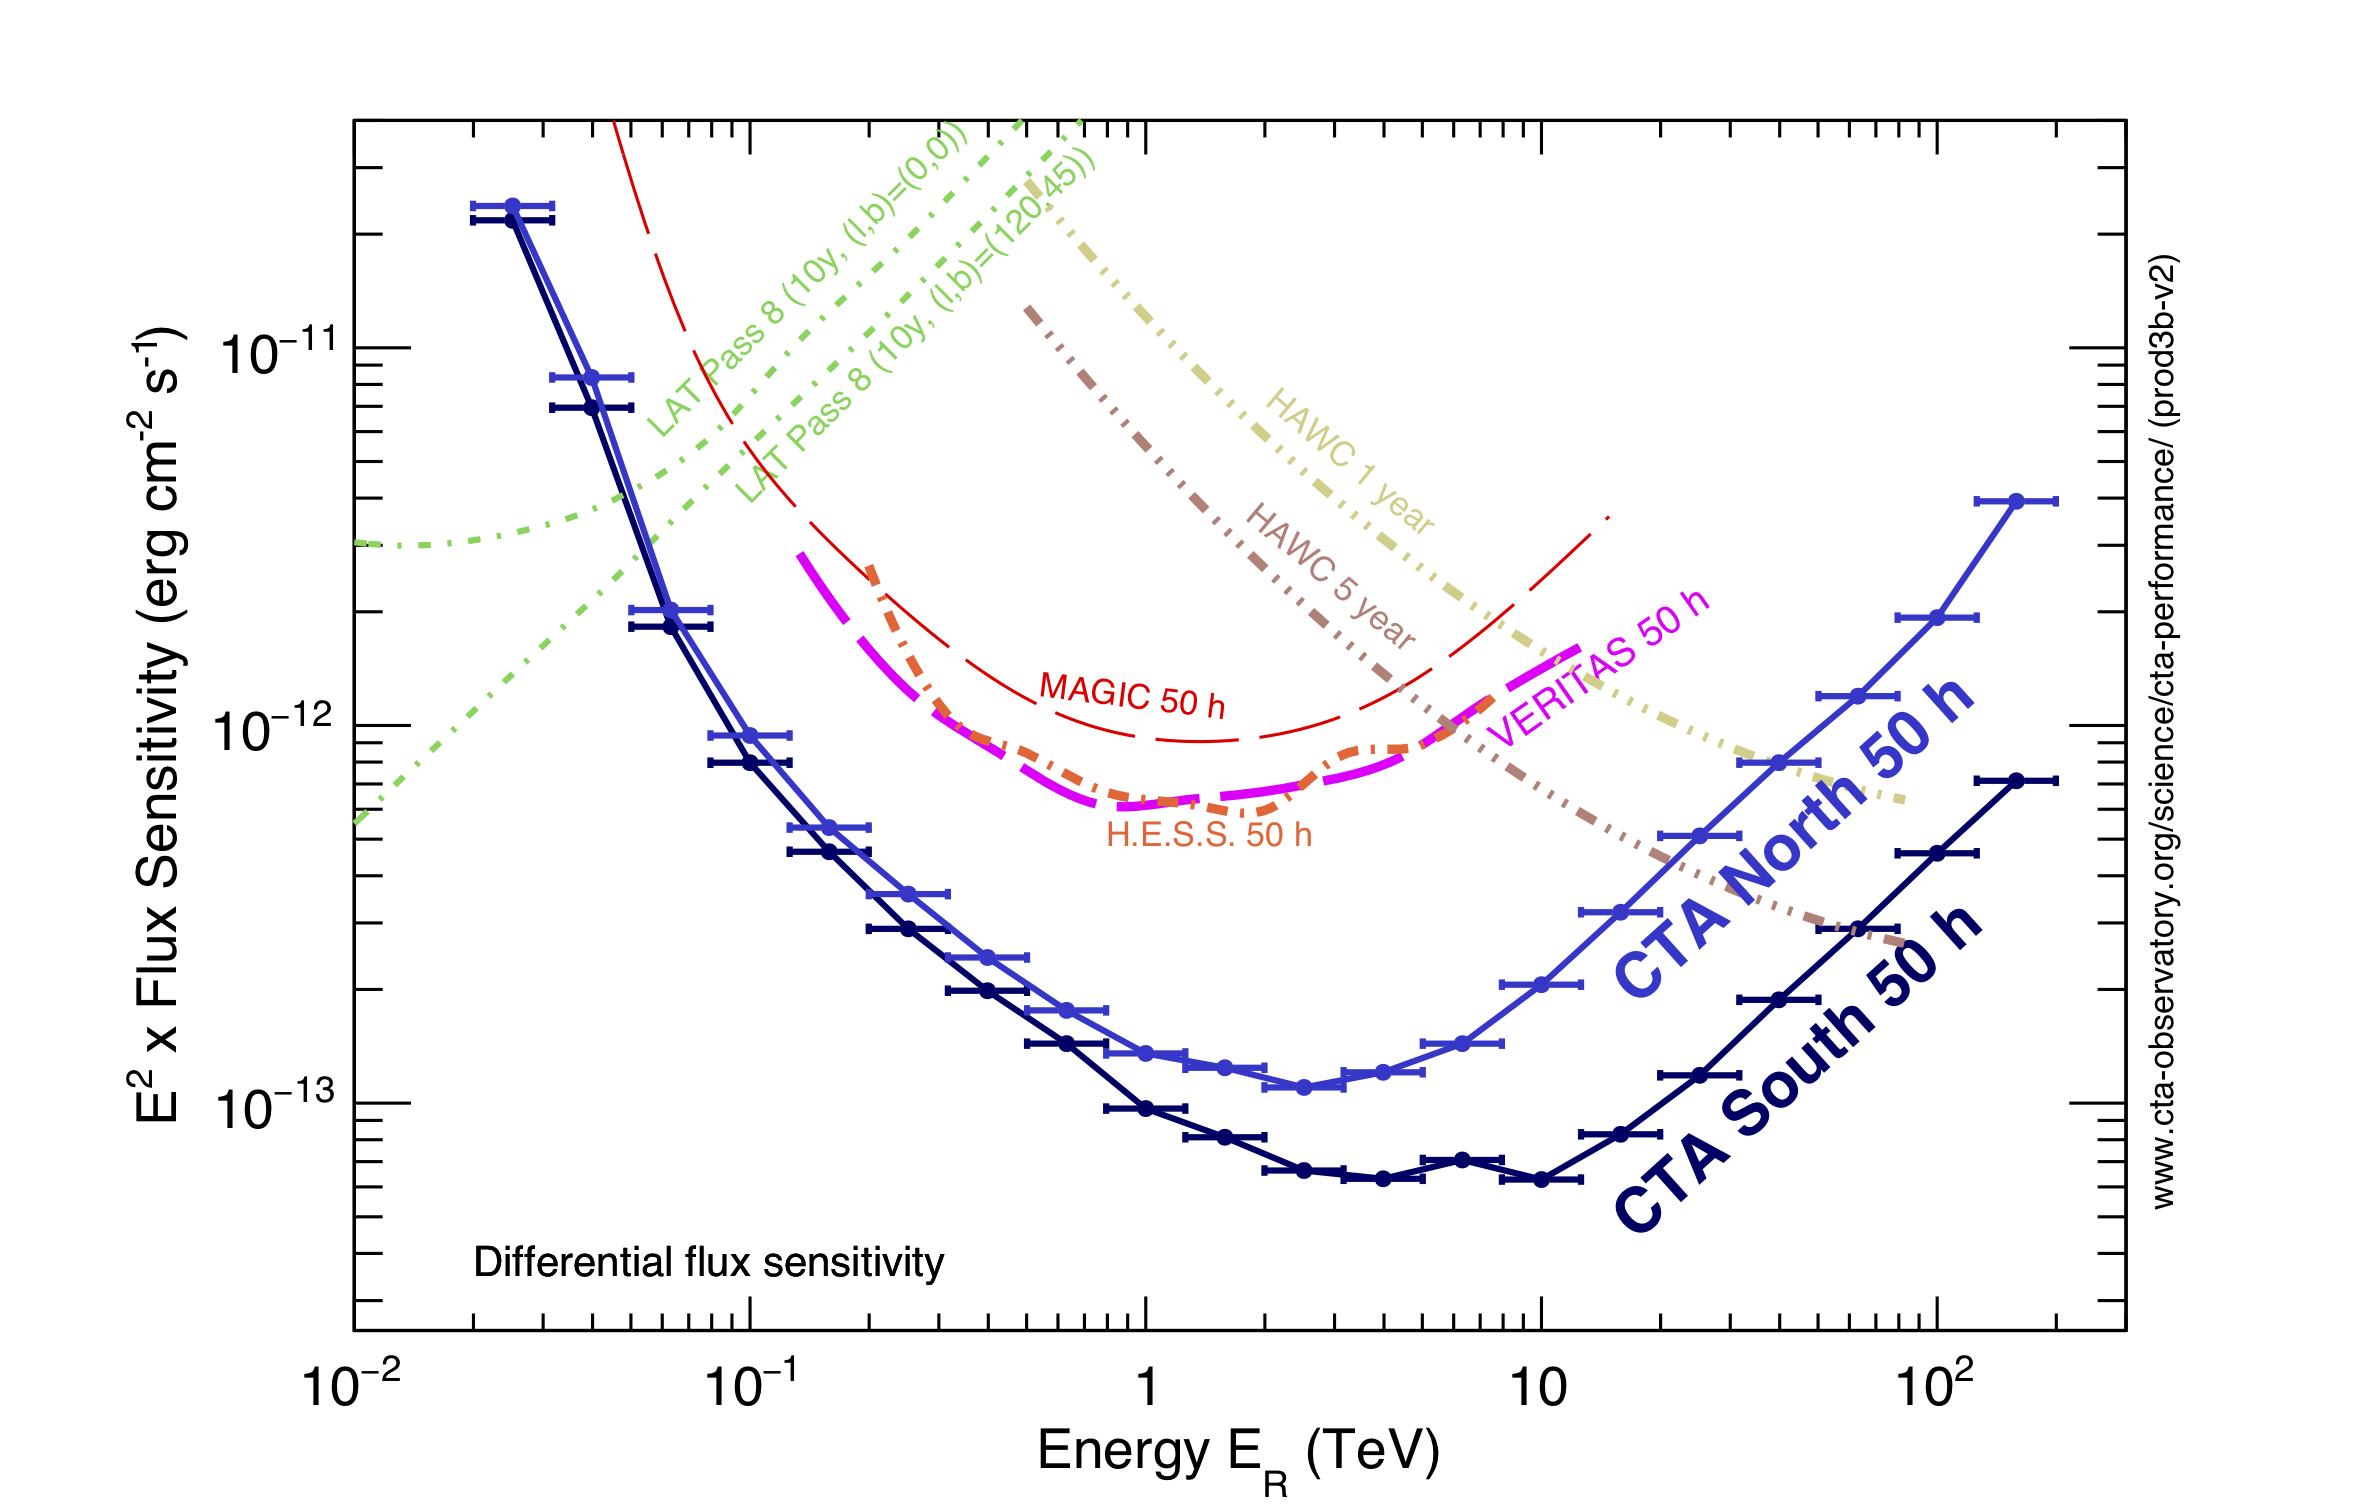
\includegraphics[width=0.9\textwidth]{images/cta_performance.png}
	\caption{A rough comparison of the expected differential sensitivity of CTA compared against
	other experiments. The differential sensitivity is defined as the
	minimum required flux to detect a point source with 5$\sigma$.
	The image is taken from the CTA-website \cite{cta_web}.}
	\label{fig:cta_performance}
\end{figure}

%\newpage
\subsection{LST}
\label{sec:lst}
The Large-Sized Telescope is going to be biggest telescope of CTA
with a mirror diameter of \SI{23}{\meter}.
It will provide the best sensitivity in the energy range from 
\SI{20}{\giga\electronvolt} to \SI{150}{\giga\electronvolt} with a field of view of \SI{4.3}{\degree}.
The camera of the LST, the LSTCamera, has \num{1855} channels 
with \num{265} photomultiplier tubes \cite{cta_web}.

The readout electronic is based on the Domino Ring Sampler 
Version 4 chip, which is also used by the MAGIC experiment
\cite{Kubo:2013pwa}. 

Since the LST is looking for the lowest energy $\gamma$-rays, it needs
very large mirror areas. At the same, time the effective detector area does 
not need to be as high as for higher energy events.
For this reason only 4 telescopes are planned per array.

The first LST has been inaugurated at the 10 October 2018 in La Palma \cite{lst_debut}.
It is foreseen to be the first telescope to be operated by the CTA Observatory.
Until the it has to undergo a critical design review to make sure the performance 
complies with the requirements and expectations.

\begin{figure}
		\centering
		\captionsetup{width=0.9\linewidth}
		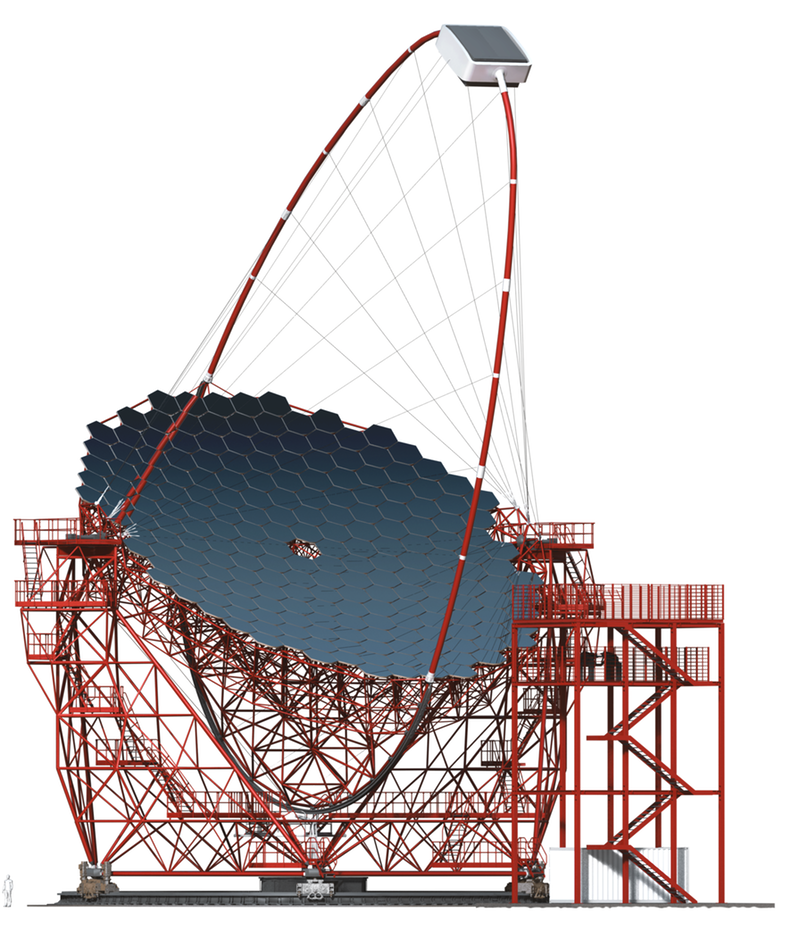
\includegraphics[width=.5\textwidth]{images/LST.png}
		\caption{
			An illustration of the Large Sized Telescope (LST) with its
			\SI{23}{\meter} diameter parabolic mirror.
			In the lower left corner a human is included for scale.
			The image can be found at the official CTA-website \cite{cta_web}.}
		\label{fig:lst}
\end{figure}

%\newpage
\subsection{MST}

\begin{wrapfigure}{R}{0.5\textwidth}
	\centering
	\captionsetup{width=0.9\linewidth}
	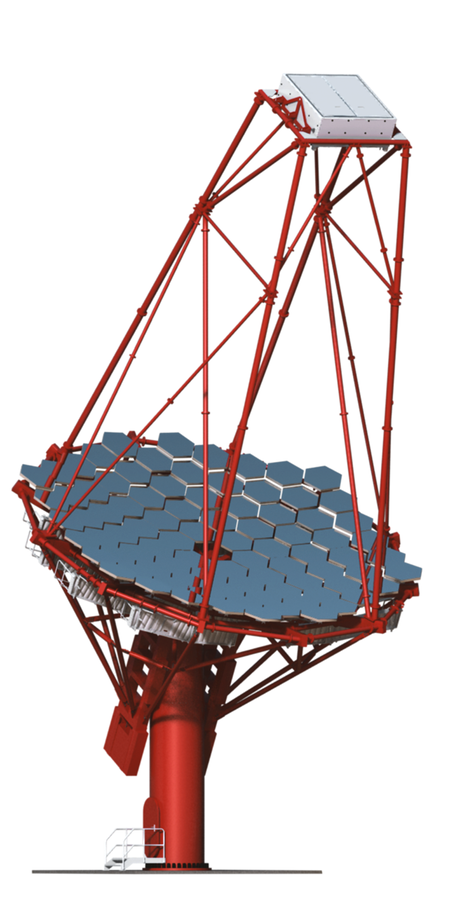
\includegraphics[width=.4\textwidth]{images/MST-1.png}
	\caption{An illustration of the Mediium Sized Telescope (MST) with its
	\SI{11.5}{\meter} diameter mirror.
	The mirror design is based on the Davies-Cotton design.
	The image can be found at the official CTA-website \cite{cta_web}.}
	\label{fig:mst}
\end{wrapfigure}

The Medium-Sized Telescopes (MST) are primarily going to look at the 
energy range from \SI{150}{\giga\electronvolt} to \SI{5}{\tera\electronvolt}.
A total of 15 telescopes on the north site and 25 telescopes at the south site 
are going to be the backbones of CTA.

Two camera designs are being tested for the MST:
The 1764 pixel FlashCam and the 1855 pixel NectarCam \cite{cta_web}.
The flashcam combines twelve PMTs to one module and features a completely
digital readout system.
The nectarcam contains an anlogue readout chip with a high-gain and a low-gain
channel. 7 PMTs are comined to one module \cite{doi:10.1063/1.4969023}.

A prototype for the MST is standing in Berlin .
Besides the camera and readout electronics it is a fully operational telescope
to validate the component design and assembly processes.
% \\
% \\
% \\
% \\
% \\
% \\
% \\
% \\
% \\
% \\

%\newpage
\subsection{SST}

The Small-Sized Telescopes (SST) will provide the sensitivity for CTA at the 
highest energies upwards from \SI{5}{\tera\electronvolt}.
An upper limit for the sensitivity is expected to be around \SI{300}{\tera\electronvolt}.

The design for the SST includes two mirrors, a \SI{4.3}{\meter} and a \SI{1.8}{\meter}
mirror, before the light hits the camera.

In contrast to the LST and MST, the SST's camera includes silicon photo-multipliers
and a total of 2048 pixels. With this the SST is going to cover a field of view 
of \SI{10.5}{\degree}.

The north array is not going to include any SSTs, the 
south array on the other hand will contain a total of 70 telescopes over
several square kilometers \cite{cta_web}.

\begin{figure}
		\centering
		\captionsetup{width=0.9\linewidth}
		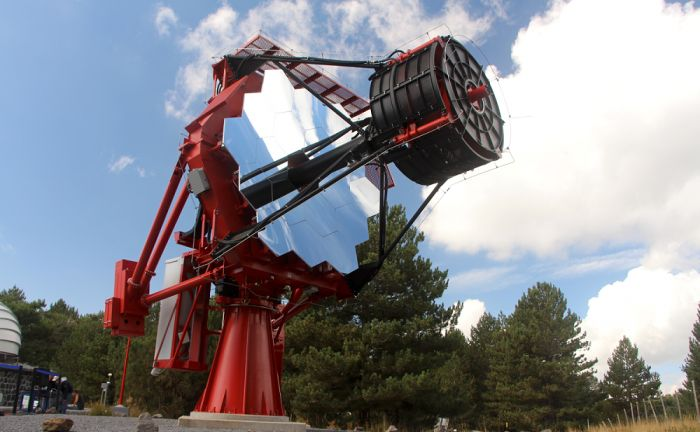
\includegraphics[width=.9\textwidth]{images/sst.jpg}
		\caption{An illustration of the Small Sized Telescope (SST) with its
		two mirrors.
		The dual-mirror Schwarzschild-Couder setup includes mirrors of
		\SI{4.3}{\meter} and \SI{1.8}{\meter} diameter.
		The image can be found at the official CTA-website \cite{cta_web}.}
		\label{fig:sst}
\end{figure}